% This is tool_support_frames.tex (Appendix D) of the OpenMP specification.
% This is an included file. See the master file for more information.
%
% When editing this file:
%
%    1. To change formatting, appearance, or style, please edit openmp.sty.
%
%    2. Custom commands and macros are defined in openmp.sty.
%
%    3. Be kind to other editors -- keep a consistent style by copying-and-pasting to
%       create new content.
%
%    4. We use semantic markup, e.g. (see openmp.sty for a full list):
%         \code{}     % for bold monospace keywords, code, operators, etc.
%         \plc{}      % for italic placeholder names, grammar, etc.
%
%    5. There are environments that provide special formatting, e.g. language bars.
%       Please use them whereever appropriate.  Examples are:
%
%         \begin{fortranspecific}
%         This is text that appears enclosed in blue language bars for Fortran.
%         \end{fortranspecific}
%
%         \begin{note}
%         This is a note.  The "Note -- " header appears automatically.
%         \end{note}
%
%    6. Other recommendations:
%         Use the convenience macros defined in openmp.sty for the minor headers
%         such as Comments, Syntax, etc.
%
%         To keep items together on the same page, prefer the use of 
%         \begin{samepage}.... Avoid \parbox for text blocks as it interrupts line numbering.
%         When possible, avoid \filbreak, \pagebreak, \newpage, \clearpage unless that's
%         what you mean. Use \needspace{} cautiously for troublesome paragraphs.
%
%         Avoid absolute lengths and measures in this file; use relative units when possible.
%         Vertical space can be relative to \baselineskip or ex units. Horizontal space
%         can be relative to \linewidth or em units.
%
%         Prefer \emph{} to italicize terminology, e.g.:
%             This is a \emph{definition}, not a placeholder.
%             This is a \plc{var-name}.
%


\chapter{Task Frame Management for the Tool Interface}
\index{task frame management}
\label{chap:frames}


   \begin{figure}[h]
    \centering
        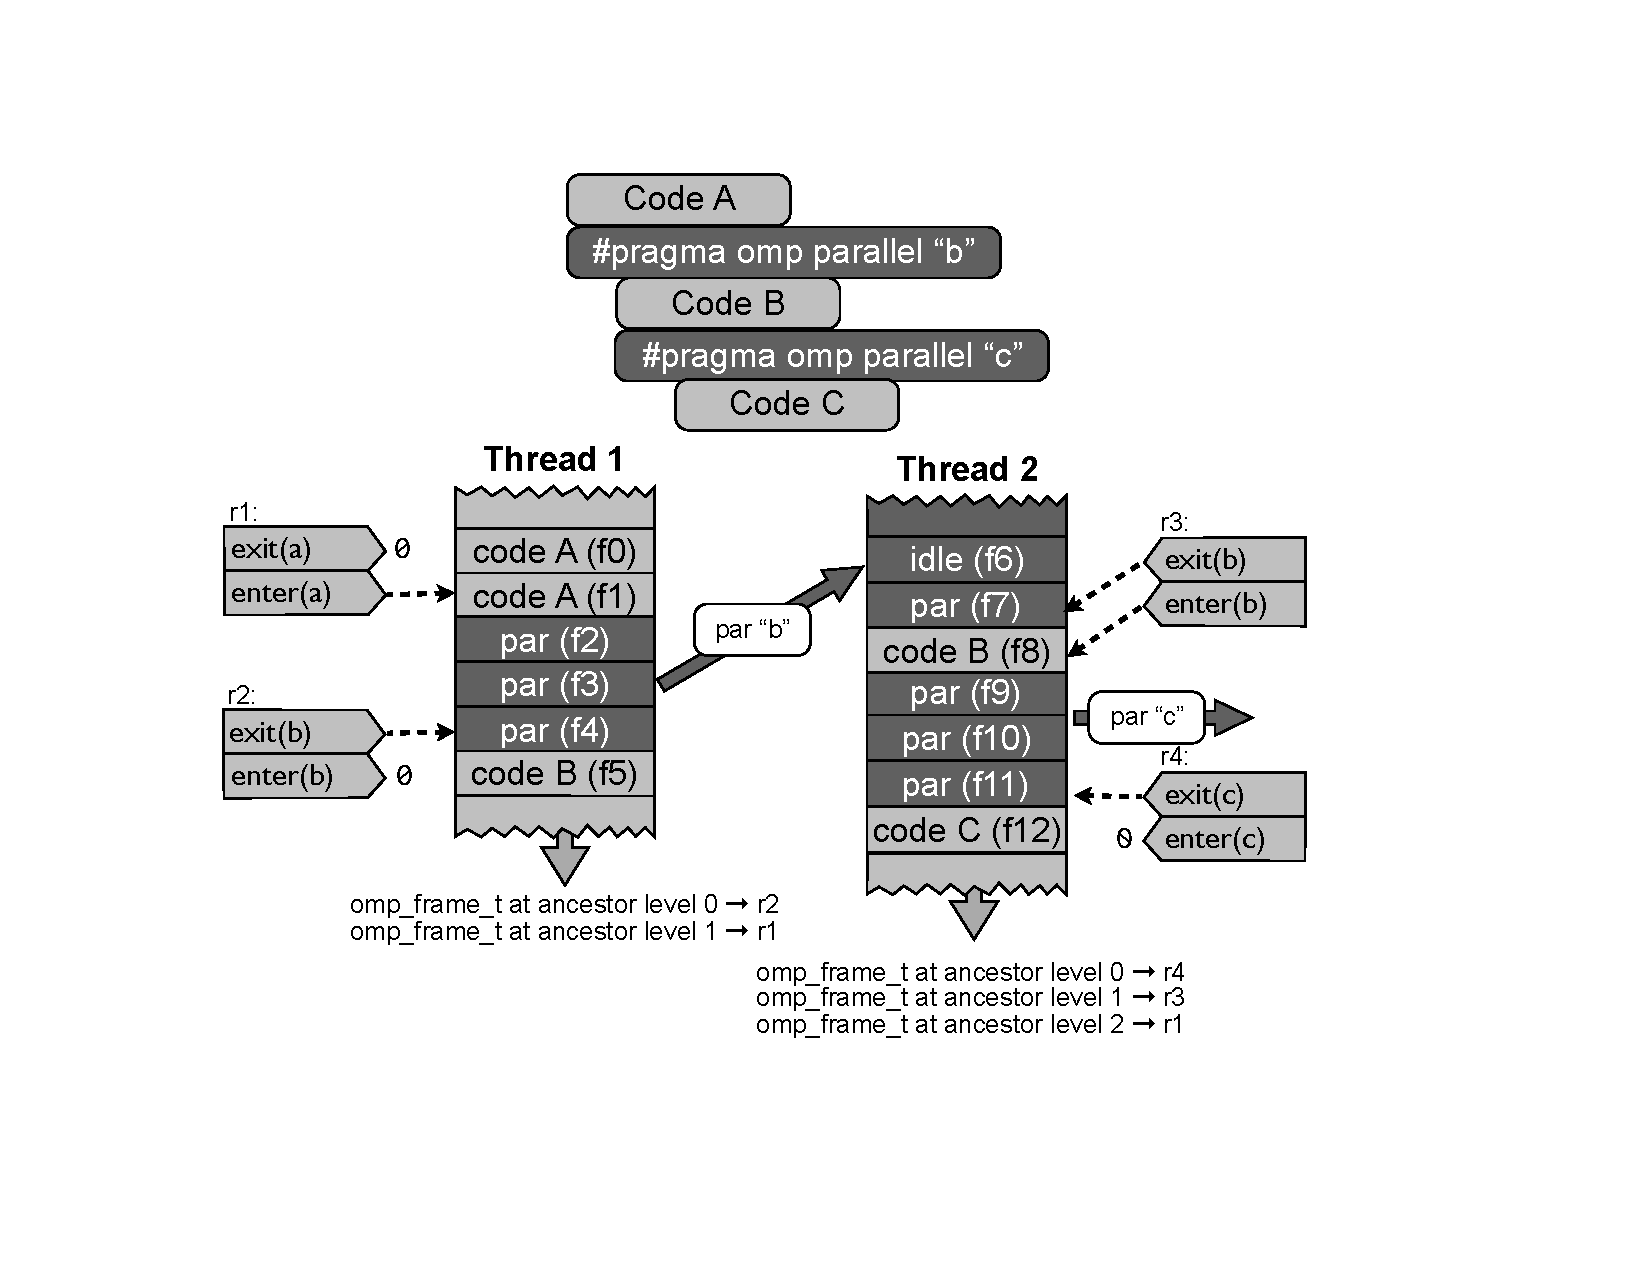
\includegraphics[width=4in]{appendices/callstack-cropped.pdf}
    \caption{Thread call stacks implementing nested parallelism
      annotated with frame information for the OMPT tool interface.}
    \label{fig:frame}
\end{figure}

The top half of Figure~\ref{fig:frame} illustrates a 
conceptualization of a program executing a nested
parallel region, where code A, B, and C represent, respectively, one
or more procedure frames of code
associated with an initial task, an outer parallel region, and an inner parallel
region. The bottom half of Figure~\ref{fig:frame} illustrates the stacks of two
threads executing the nested parallel region. 
In the illustration, stacks grow downward---a call to a function adds
a new frame to the stack below the frame of its caller.
When thread 1 encounters the outer-parallel
region ``b", it calls a routine in the OpenMP runtime to
create a new parallel region. The OpenMP runtime sets the
\plc{enter_frame} field in the \code{omp_frame_t} for the initial
task executing code A to the canonical frame address of frame f1---the user frame in the initial task
that calls the runtime. The \code{omp_frame_t} for the initial task
is labeled \plc{r1} in Figure~\ref{fig:frame}. In this figure, three
consecutive runtime system frames, labeled ``par'' with frame
identifiers f2--f4, are on the stack.  Before starting the implicit
task for parallel region ``b" in thread 1, the runtime sets the
\plc{exit_frame} in the implicit task's \code{omp_frame_t} (labeled
\plc{r2}) to the canonical frame address of frame f4. Execution of application code for parallel region
``b'' begins on thread 1 when the runtime system invokes application
code B (frame f5) from frame f4.

Let us focus now on thread 2, an OpenMP thread. Figure~\ref{fig:frame}
shows this worker executing work for the outer-parallel region ``b."
On the OpenMP thread's stack is a runtime frame labeled ``idle,''
where the OpenMP thread waits for work.  When work becomes available,
the runtime system invokes a function to dispatch it. While
dispatching parallel work might involve a chain of several calls, here
we assume that the length of this chain is 1 (frame f7).  Before
thread 2 exits the runtime to execute an implicit task for parallel
region ``b,'' the runtime sets the \plc{exit_frame} field of the
implicit task's \code{omp_frame_t} (labeled \plc{r3}) to the canonical frame address of frame f7.
When thread 2 later encounters the inner-parallel region ``c," as
execution returns to the runtime, the runtime fills in the
\plc{enter_frame} field of the current task's \code{omp_frame_t}
(labeled \plc{r3}) to the canonical frame address of frame f8---the frame that invoked the
runtime. Before the task for parallel region ``c'' is invoked on
thread 2, the runtime system sets the \plc{exit_frame} field of the
\code{omp_frame_t} (labeled \plc{r4}) for the implicit task for
``c'' to the canonical frame address of frame f11. Execution of application code for parallel region
``c'' begins on thread 2 when the runtime system invokes application
code C (frame f12) from frame f11.


Below the stack for each thread in Figure~\ref{fig:frame}, the figure
shows the \code{omp_frame_t} information obtained by calls to
\code{ompt_get_task_info} made on each thread for the stack state
shown. We show the ID of the \code{omp_frame_t} object returned at
each ancestor level. Note that thread 2 has task frame information for
three levels of tasks, whereas thread 1 has only two.

\crossreferences
\begin{itemize}
\item \code{omp_frame_t}, see \specref{sec:omp_frame_t}.
\item \code{ompt_get_task_info_t}, see \specref{sec:ompt_get_task_info_t}.
\end{itemize}


% This is the end of appendix-frames.tex

